\documentclass[12pt]{article}
\usepackage[table,xcdraw]{xcolor}
\usepackage{multirow}
\usepackage{pdflscape}
\usepackage{amsmath}
\usepackage{amsfonts}
\usepackage{float}
\usepackage{fancyhdr}
\usepackage{graphicx}
\usepackage{hyperref}
\usepackage{indentfirst}
\usepackage{url}
\usepackage{subfig}
\usepackage[top=.75in, left=.75in, right=.75in, bottom=1in]{geometry}
\usepackage{gensymb}
\hypersetup{
    colorlinks=true,
    linkcolor=blue,
    filecolor=magenta,      
    urlcolor=cyan,
    pdftitle={Overleaf Example},
    pdfpagemode=FullScreen,
    }
%\usepackage[utf8]{vietnam}

% For algorithm
\usepackage{algorithm}
\usepackage{algpseudocode}

% ============ CODE ============
\usepackage{listings} 
\usepackage{xcolor}
\definecolor{codegreen}{rgb}{0,0.6,0}
\definecolor{codegray}{rgb}{0.5,0.5,0.5}
\definecolor{codepurple}{rgb}{0.58,0,0.82}
\definecolor{backcolour}{rgb}{0.95,0.95,0.92}

% Styling for the code.
\lstdefinestyle{mystyle}{
    backgroundcolor=\color{backcolour},   
    commentstyle=\color{codegreen},
    keywordstyle=\color{magenta},
    numberstyle=\tiny\color{codegray},
    stringstyle=\color{codepurple},
    basicstyle=\ttfamily\footnotesize,
    breakatwhitespace=false,         
    breaklines=true,                 
    captionpos=b,                    
    keepspaces=true,                 
    numbers=left,                    
    numbersep=5pt,                  
    showspaces=false,                
    showstringspaces=false,
    showtabs=false,                  
    tabsize=2
}
\lstset{style=mystyle}

% Disable indentation on new paragraphs
\setlength{\parindent}{0pt}

% Optional: graphic path
% \graphicspath{PATH_TO_GRAPHIC_FOLDER}

% To use Times font family, uncomment this row
% \usepackage{mathptmx}

% To use roman section / subsection, uncomment these rows
% \renewcommand{\thesection}{\Roman{section}}
% \renewcommand{\thesubsection}{\thesection.\Roman{subsection}}

% Define course name, report name and report title.
\newcommand{\coursename}{Data Structures and Algorithms}
\newcommand{\reportname}{Exercise 1: Implementing Stack and Queue from scratch}
\newcommand{\reporttitle}{Report}

\newcommand{\studentname}{Nguyen Le Ho Anh Khoa - 23127211}
\newcommand{\teachername}{Bui Duy Dang \\ Truong Tan Khoa \\ Nguyen Thanh Tinh}

% ============ HEADER AND FOOTER ============
% Header length
\setlength{\headheight}{29.43912pt}

% Footer page number would be on the lower-right corner
\pagestyle{fancy}
\fancyfoot{}
\fancyfoot[R]{Page \thepage}

\lhead{\reportname}
\rhead{VNUHCM-US\\
\coursename
}
% Remove the \leftfooter command from the footer definition
\lfoot{}

%Footer page number for landscape
\fancypagestyle{lscape}{
\fancyhf{}
\fancyfoot[R]{Page \thepage}
\renewcommand{\headrulewidth}{0pt} 
  \renewcommand{\footrulewidth}{0pt}
}



% ============ DOCUMENT ============
\begin{document}
\begin{titlepage}
\newcommand{\HRule}{\rule{\linewidth}{0.5mm}}
\centering

\textsc{\LARGE vietnam national university of \\ho chi minh city}\\[0.8cm]
\textsc{\Large university of science}\\[0.4cm]
\textsc{\large faculty of information technology}\\[0.4cm]

\HRule \\[0.4cm]
{ 
\Large{\bfseries{\reporttitle}}\\[0.4cm]
\huge{\bfseries{\reportname}}
}\\[0.4cm]
\HRule \\[0.4cm]

\textbf{\large Course name: \coursename}\\[0.4cm]
\textbf{\large CSC10004\textunderscore23CLC09} \\ [0.7cm]
\begin{minipage}[t]{0.4\textwidth}
\begin{flushleft} \large
\emph{Students:}\\
\studentname
\end{flushleft}
\end{minipage}
~
\begin{minipage}[t]{0.4\textwidth}
\begin{flushright} \large
\emph{Teacher:} \\
\teachername
\end{flushright}
\end{minipage}\\[0.7cm]

{\large \today}\\[1cm]


\includegraphics[scale=1.1]{img/hcmus-logo.png}\\[0cm] 

\vfill
\end{titlepage}
	
\tableofcontents
\pagebreak
\section{Student Information}
Class: 23CLC09 \\
Student ID: 23127211 \\
Full name: Nguyen Le Ho Anh Khoa
\pagebreak
\section{Detailed Experiments}
\label{sec:detailedExperiments}

\subsection{Linear Probing}


\subsubsection{Add key:}
The order insert key to the Hash Table by Linear Probing is as follows: [one; 1], [two; 2], [three; 3], [four; 4], [five; 5], [one; 111], [two; 222]. The size of the Hash Table is 5. The Hash Table is shown in the figure below:

\begin{figure}[H]
	\centering
	\subfloat[\centering Add new]{{\includegraphics[width=7cm]{img/Linear/addnew.PNG} }}%
	\qquad
	\subfloat[\centering Update]{{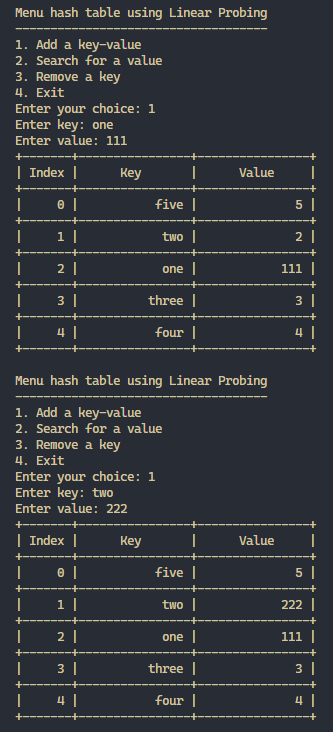
\includegraphics[width=7cm]{img/Linear/updateValue.PNG} }}%
	\caption{Add new by key by Linear Probing}%
\end{figure}

\subsubsection{Search key (Use the Hash Table added as above 3.1.1):}
\begin{figure}[H]
	\centering
	\subfloat[\centering Found]{{\includegraphics[width=7cm]{img/Linear/Found.PNG} }}%
	\qquad
	\subfloat[\centering Not Found]{{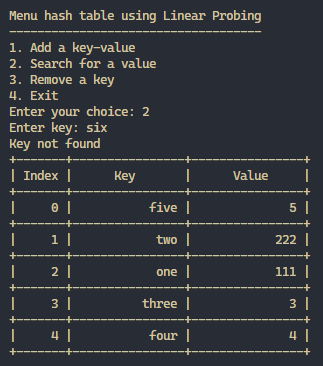
\includegraphics[width=7cm]{img/Linear/Not found.PNG} }}%
	\caption{Search value by key by Linear Probing (size=5)}%
\end{figure}

\subsubsection{Remove key (Use the Hash Table added as above 3.1.1):}
\begin{figure}[H]
	\centering
	\subfloat[\centering Removed]{{\includegraphics[width=7cm]{img/Linear/removed.PNG} }}%
	\qquad
	\subfloat[\centering Not Found]{{\includegraphics[width=7cm]{img/Linear/removeNotFound.PNG} }}%
	\caption{Remove value by key by Linear Probing}%
\end{figure}

\subsubsection{Experiments Linear Probing and Linear Search Algorithms}
\begin{figure}[H]
	\centering
	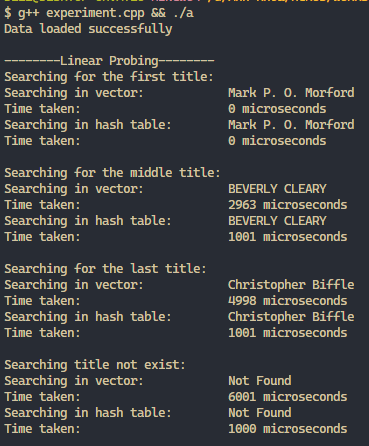
\includegraphics[width=0.7\linewidth]{img/Linear/Compare.PNG}
	\caption{Compare time Linear Probing Search and Linear Search Algorithms}
\end{figure}

\begin{itemize}
	\item The time complexity of Linear Probing Search is O(n)
	\item The time complexity of Linear Search Algorithms is O(n).
\end{itemize}
But in the most cases, using Linear Probing Search in Hash Table is faster than using Linear Search Algorithms in normal vector.

\pagebreak
\subsection{Quadratic Probing}


\subsubsection{Add key:}
The order insert key to the Hash Table by Quadratic Probing is as follows: [one; 1], [two; 2], [three; 3], [four; 4], [five; 5], [one; 111], [two; 222]. The size of the Hash Table is 5. But after added the key [three; 3], the size of the Hash Table is 10 by rehashing. However, this condition can be met even if there are still empty slots available, due to the nature of quadratic probing. The Hash Table is shown in the figure below:

\begin{figure}[H]
	\centering
	\subfloat[\centering Add new]{{\includegraphics[width=7cm]{img/Quadratic/addnew.PNG} }}%
	\qquad
	\subfloat[\centering Update]{{\includegraphics[width=7cm]{img/Quadratic/update.PNG}}}%
	\caption{Add new key by Quadratic Probing (size=5)}%
\end{figure}

\subsubsection{Search key (Use the Hash Table added as above 3.2.1):}
\begin{figure}[H]
	\centering
	\subfloat[\centering Found]{{\includegraphics[width=7cm]{img/Quadratic/Found.PNG} }}%
	\qquad
	\subfloat[\centering Not Found]{{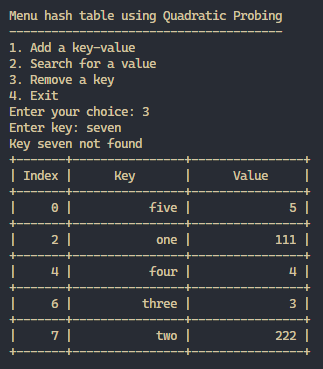
\includegraphics[width=7cm]{img/Quadratic/notFound.PNG} }}%
	\caption{Search value by key by Quadratic Probing (size=5)}%
\end{figure}

\subsubsection{Remove key (Use the Hash Table added as above 3.2.1):}
\begin{figure}[H]
	\centering
	\subfloat[\centering Removed]{{\includegraphics[width=7cm]{img/Quadratic/removed.PNG} }}%
	\qquad
	\subfloat[\centering Not Found]{{\includegraphics[width=7cm]{img/Quadratic/removeNotFound.PNG} }}%
	\caption{Remove value by key by Quadratic Probing}%
\end{figure}

\subsubsection{Experiments Quadratic Probing and Linear Search Algorithms}
\begin{figure}[H]
	\centering
	\includegraphics[width=0.7\linewidth]{img/Quadratic/compare.PNG}
	\caption{Compare time Quadratic Probing and Linear Search Algorithms}
\end{figure}

\begin{itemize}
	\item The time complexity of Quadratic Probing Search is O(n)
	\item The time complexity of Linear Search Algorithms is O(n).
\end{itemize}
But in the most cases, using Quadratic Probing Search in Hash Table is faster than using Linear Search Algorithms in normal vector.\\

\pagebreak
\subsection{Chaining using Linked List}

\subsubsection{Add key:}
The order insert key to the Hash Table by Chaining using Linked List is as follows: [one; 1], [two; 2], [three; 3], [four; 4], [five; 5], [one; 111], [two; 222]. The size of the Hash Table is 5. The Hash Table is shown in the figure below:

\begin{figure}[H]
	\centering
	\subfloat[\centering Add new]{{\includegraphics[width=7cm]{img/ChainingLinkedList/addnew.PNG} }}%
	\qquad
	\subfloat[\centering Update]{{\includegraphics[width=7cm]{img/ChainingLinkedList/update.PNG} }}%
	\caption{Add new by key by Chaining using Linked List}%
\end{figure}

\subsubsection{Search key (Use the Hash Table added as above 3.3.1):}
\begin{figure}[H]
	\centering
	\subfloat[\centering Found]{{\includegraphics[width=7cm]{img/ChainingLinkedList/found.PNG} }}%
	\qquad
	\subfloat[\centering Not Found]{{\includegraphics[width=7cm]{img/ChainingLinkedList/notfound.PNG} }}%
	\caption{Search value by key by Chaining using Linked List}%
\end{figure}

\subsubsection{Remove key (Use the Hash Table added as above 3.3.1):}
\begin{figure}[H]
	\centering
	\subfloat[\centering Removed]{{\includegraphics[width=7cm]{img/ChainingLinkedList/found.PNG} }}%
	\qquad
	\subfloat[\centering Not Found]{{\includegraphics[width=7cm]{img/ChainingLinkedList/removeNotFound.PNG} }}%
	\caption{Remove value by key by Chaining Using Linked List}%
\end{figure}

\subsubsection{Experiments Chaining Using Linked List and Linear Search Algorithms}
\begin{figure}[H]
	\centering
	\includegraphics[width=0.7\linewidth]{img/ChainingLinkedList/compare.PNG}
	\caption{Compare time Chaining using Linked List Search and Linear Search Algorithms}
\end{figure}

\begin{itemize}
	\item The time complexity of Chaining using Linked List Search is O(n)
	\item The time complexity of Linear Search Algorithms is O(n).
\end{itemize}
But in the most cases, using Chaining using Linked List Search in Hash Table is faster than using Linear Search Algorithms in normal vector.

\pagebreak
\subsection{Chaining using AVL Tree}
\subsubsection{Add key:}
The order insert key to the Hash Table by Chaining using AVL Tree is as follows: [one; 1], [two; 2], [three; 3], [four; 4], [five; 5], [one; 111], [two; 222]. The size of the Hash Table is 5. The Hash Table is shown in the figure below:

\begin{figure}[H]
	\centering
	\subfloat[\centering Add new]{{\includegraphics[width=7cm]{img/ChainingAVL/addnew.PNG} }}%
	\qquad
	\subfloat[\centering Update]{{\includegraphics[width=7cm]{img/ChainingAVL/update.PNG} }}%
	\caption{Add new by key by Chaining using AVL Tree}%
\end{figure}

\subsubsection{Search key (Use the Hash Table added as above 3.4.1):}
\begin{figure}[H]
	\centering
	\subfloat[\centering Found]{{\includegraphics[width=7cm]{img/ChainingAVL/found.PNG} }}%
	\qquad
	\subfloat[\centering Not Found]{{\includegraphics[width=7cm]{img/ChainingAVL/notfound.PNG} }}%
	\caption{Search value by key by CChaining Using AVL Tree}%
\end{figure}

\subsubsection{Remove key (Use the Hash Table added as above 3.4.1):}
\begin{figure}[H]
	\centering
	\subfloat[\centering Removed]{{\includegraphics[width=7cm]{img/ChainingAVL/removed.PNG} }}%
	\qquad
	\subfloat[\centering Not Found]{{\includegraphics[width=7cm]{img/ChainingAVL/removeNotFound.PNG} }}%
	\caption{Remove value by key by Chaining Using AVL Tree}%
\end{figure}

\subsubsection{Experiments Chaining using AVL Tree and Linear Search Algorithms}
\begin{figure}[H]
	\centering
	\includegraphics[width=0.7\linewidth]{img/ChainingAVL/compare.PNG}
	\caption{Compare time Chaining using AVL Tree Search and Linear Search Algorithms}
\end{figure}

\begin{itemize}
	\item The time complexity of Chaining using AVL Tree Search is O(logn)
	\item The time complexity of Linear Search Algorithms is O(n).
\end{itemize}
So in the most cases, using Chaining using AVL Tree Search in Hash Table is faster than using Linear Search Algorithms in normal vector.


\pagebreak
\subsection{Double Hashing}

\subsubsection{Add key:}
The order insert key to the Hash Table size = 5 by Double Hashing is as follows: [one; 1], [two; 2], [three; 3], [four; 4], [five; 5], [one; 111], [two; 222].The Hash Table is shown in the figure below:

\begin{figure}[H]
	\centering
	\subfloat[\centering Add new]{{\includegraphics[width=7cm]{img/DoubleHash/addnew.PNG} }}%
	\qquad
	\subfloat[\centering Update]{{\includegraphics[width=7cm]{img/DoubleHash/update.PNG}}}%
	\caption{Add new key by Quadratic Probing (size=5)}%
\end{figure}

\subsubsection{Search key (Use the Hash Table added as above 3.5.1):}
\begin{figure}[H]
	\centering
	\subfloat[\centering Found]{{\includegraphics[width=7cm]{img/DoubleHash/found.PNG} }}%
	\qquad
	\subfloat[\centering Not Found]{{\includegraphics[width=7cm]{img/DoubleHash/notfound.PNG} }}%
	\caption{Search value by key by Quadratic Probing (size=5)}%
\end{figure}

\subsubsection{Remove key (Use the Hash Table added as above 3.5.1):}
\begin{figure}[H]
	\centering
	\subfloat[\centering Removed]{{\includegraphics[width=7cm]{img/DoubleHash/removed.PNG} }}%
	\qquad
	\subfloat[\centering Not Found]{{\includegraphics[width=7cm]{img/DoubleHash/removeNotFound.PNG} }}%
	\caption{Remove value by key by Double Hashing}%
\end{figure}

\subsubsection{Experiments Double Hashing and Linear Search Algorithms}
\begin{figure}[H]
	\centering
	\includegraphics[width=0.7\linewidth]{img/DoubleHash/compare.PNG}
	\caption{Compare time Double Hashing Search and Linear Search Algorithms}
\end{figure}

\begin{itemize}
	\item The time complexity of Double Hashing Search is O(n)
	\item The time complexity of Linear Search Algorithms is O(n).
\end{itemize}
But in the most cases, using Double Hashing Search in Hash Table is faster than using Linear Search Algorithms in normal vector.\\

When run with large dataset, Hash Table by Double Hashing need to rehash because the condition \textbf{ if (i == capacity)} is used to determine if the table is full. However, this condition can be met even if there are still empty slots available, due to the nature of quadratic probing.

\section{Đánh giá}
\subsection{Bảng tự đánh giá các yêu cầu đã hoàn thành}

\begin{center}
\begin{table}[H]
    \centering
    \caption{Bảng tự đánh giá bài 1}
    \renewcommand{\arraystretch}{1.4}
    \begin{tabular}{|l|p{\dimexpr0.6\linewidth-2\tabcolsep}|c|}
    \hline
    \textbf{STT} & \textbf{Yêu cầu}            & \textbf{Mức độ hoàn thành} \\ \hline
    1            &  Nhập vào số nguyên X (4 byte) có dấu hãy "đọc" dãy bit nhị phân của X và xuất ra màn hình.       & 100\%          \\ \hline
    2            & Cho mảng 1 chiều A gồm 32 phần tử là các số 0 hoặc 1. Hãy xây dựng số nguyên X 4 byte có các bit giống với các phần tử mảng A, sau đó xuất X ra màn hình.
    & 100\%          \\ \hline
                & \textbf{Tổng cộng}               &\textbf{100\%}           \\ \hline
    \end{tabular}
    \label{tab:mytable}
\end{table}

  \begin{table}[H]
        \centering
        \caption{Bảng tự đánh giá bài 2}
        \renewcommand{\arraystretch}{1.4}
        \begin{tabular}{|l|p{\dimexpr0.6\linewidth-2\tabcolsep}|c|}
        \hline
        \textbf{STT} & \textbf{Yêu cầu}            & \textbf{Mức độ hoàn thành} \\ \hline
        1            &  Thực hiện phép tính cộng   & 100\%          \\ \hline
        2            &  Thực hiện phép tính trừ      & 100\%          \\ \hline
        3            &  Thực hiện phép tính nhân theo thuật toán Booth      & 100\%          \\ \hline
        4            &  Thực hiện phép tính chia lấy phần nguyên      & 100\%          \\ \hline
        5            &  Thực hiện phép tính chia lấy phần dư      & 100\%          \\ \hline
                    & \textbf{Tổng cộng}               &\textbf{100\%}           \\ \hline
      \end{tabular}
        \label{tab:mytable2}
  \end{table}
\end{center}

\subsection{Đánh giá tổng thể mức độ hoàn thành của bài nộp}

Bài nộp đã hoàn thành đầy đủ các yêu cầu đề ra trong bài tập. Tất cả các yêu cầu đều đã được cài đặt và kiểm thử thành công. Tổng thể, bài nộp đã hoàn thành 100\% các yêu cầu đề ra.

\section{Exercise Feedback}

\subsection{What have I learned}
\begin{itemize}
    \item In the past, my approach was sequential programming, but this task has broadened my knowledge to include the fundamentals of object-oriented programming.
    \item I’ve acquired skills in creating reports with \LaTeX.
    \item I’ve employed Github as a vault for my source code and reports, all of which are securely stored in \href{https://github.com/KhoaNguyen-HCMUS/HCMUS-course}{my personal repository}.
\end{itemize}
\subsection{What was my difficult}
\begin{itemize}
    \item At the outset, my journey with programming was fraught with difficulties due to my unfamiliarity with object-oriented programming. However, my comprehension has been greatly enhanced after delving into a plethora of resources available on the internet. \cite{OOP_in_C++}
    \item I encountered some difficulties when writing function about AVL tree. However, after a period of debugging and contemplation, I successfully resolved the issues. \cite{AVL_Tree}
    \item I had a hard time understanding the concept of hash tables, but after a period of research and experimentation, I was able to grasp the fundamentals.
    \item Measuring the time complexity of the algorithms was a challenging task, but I was able to overcome it by using the Chrono library in C++. \cite{Measure_time_in_C++}
    \item Lastly, my English proficiency isn’t quite up to par yet, so there’s a possibility that this report contains some grammatical errors.
\end{itemize}


\bibliographystyle{plain}
\bibliography{content/bibl}


\end{document}